\documentclass[12pt]{article}

\usepackage{bbm}
\usepackage{fancyhdr}
\usepackage{titling}
\usepackage{enumitem}
\usepackage{amsmath}
\usepackage{dsfont}
\usepackage{amsfonts}
\usepackage{amssymb}
\usepackage{amsthm}
\usepackage{geometry}
\usepackage{tikz}
\usepackage{algorithm}
\usepackage{algpseudocode}
\geometry{verbose,tmargin=1in,bmargin=1in,lmargin=1in,rmargin=1in}
\renewcommand{\vec}[1]{\mathbf{#1}}
\newcommand{\dec}{\text{dec}}
\newcommand{\divi}{\mathbin{\textnormal{div}}}
\title{Homework 1}
\author{Satvik Prasad}
\date{}
\newtheorem{lemma}{Lemma}[section]
\fancypagestyle{plain}{%
  \fancyhf{}
  \fancyhead[L]{\theauthor}
  \fancyhead[R]{\thedate}
}
\pagestyle{plain}
\makeatletter
\def\@maketitle{%
  \newpage
  \null
  \vskip 1em%
  \begin{center}%
    \let \footnote \thanks
    {\LARGE \@title \par}%
    \vskip 1em%
  \end{center}%
  \par
\vskip 1em}
\makeatother
\usepackage{cmbright}

\newcommand{\mat}[1]{\mathbf{#1}}

% ---------- Probability theory ----------
% Core operators (optional argument-free; use as \E{X}, \Var{X}, \Cov{X}{Y})
\DeclareMathOperator{\EOp}{\mathbb{E}}
\DeclareMathOperator{\VarOp}{Var}
\DeclareMathOperator{\CovOp}{Cov}
\DeclareMathOperator{\CorrOp}{Corr}

\renewcommand{\P}[1]{\mathbb{P}\left(#1\right)}        % \P{A}
\newcommand{\E}[1]{\EOp\left[#1\right]}                % \E{X}
\newcommand{\Var}[1]{\VarOp\left(#1\right)}            % \Var{X}
\newcommand{\Cov}[2]{\CovOp\left(#1,\,#2\right)}       % \Cov{X}{Y}
\newcommand{\Corr}[2]{\CorrOp\left(#1,\,#2\right)}     % \Corr{X}{Y}
\newcommand{\SD}[1]{\operatorname{SD}\left(#1\right)}  % \SD{X}

% Subscripted versions, e.g. \Esub{\theta}{X}, \Psub{\theta}{A}
\newcommand{\Esub}[2]{\EOp_{#1}\left[#2\right]}
\newcommand{\Psub}[2]{\mathbb{P}_{#1}\left(#2\right)}

% Conditioning, indicators, independence
\newcommand{\given}{\,\middle|\,}                      % \E{X \given Y}
\newcommand{\ind}[1]{\mathbbm{1}\left\{#1\right\}}     % \ind{X > 0}
\newcommand{\indep}{\perp\!\!\!\perp}                  % X \indep Y
\newcommand{\iid}{\overset{\text{iid}}{\sim}}          % X_i \iid \Normal(0,1)

% Convergence
\newcommand{\convp}{\xrightarrow{\;p\;}}               % in probability
\newcommand{\convd}{\xrightarrow{\;d\;}}               % in distribution
\newcommand{\convas}{\xrightarrow{\text{a.s.}}}        % almost surely
\newcommand{\convLp}[1]{\xrightarrow{L^{#1}}}          % in L^p

% Probability spaces
\newcommand{\F}{\mathcal{F}}                           % sigma-algebra
\newcommand{\B}{\mathcal{B}}                           % Borel sigma-algebra
\newcommand{\pspace}{(\Omega, \F, \mathbb{P})}

% Common distributions
\newcommand{\Normal}{\mathcal{N}}
\newcommand{\Bern}{\operatorname{Bernoulli}}
\newcommand{\Bin}{\operatorname{Binomial}}
\newcommand{\Pois}{\operatorname{Poisson}}
\newcommand{\Unif}{\operatorname{Uniform}}
\newcommand{\Exp}{\operatorname{Exp}}
\newcommand{\Geom}{\operatorname{Geometric}}
\newcommand{\Gam}{\operatorname{Gamma}}
\newcommand{\Beta}{\operatorname{Beta}}

% Number sets
\newcommand{\R}{\mathbb{R}}
\newcommand{\N}{\mathbb{N}}
\newcommand{\Z}{\mathbb{Z}}


\begin{document}
\begin{enumerate}
  \item To show that Special Clique is NP-hard, we reduce Clique to
    Special Clique. Given a graph $G$ on which we wish to determine
    whether there exists a $k$-clique graph, modify the graph $G \to
    G^\star$ by duplicating every vertex $v \to v, v^\star$ (without
    modifying edge set) and constructing edge $(v, v^\star).$

    For now, consider the case where $k > 2.$

    Assume that the graph $G^\star$ has a special $k$-clique, and let
    this clique be $K_k.$ Then, if $k > 2$ any duplicated vertex
    $v^\star$ cannot be a part of this clique, since the degree of
    $v^\star$ is $1,$ and any vertex in the clique must have degree
    $k - 1.$ Hence, $G$ has a $k$-clique if $G^\star$ has a special $k$-clique.

    Conversely, if $G$ has a $k$-clique, then $G^\star$ has a special
    $k$-clique by assigning the vertices $v'$ to be the duplicated
    vertices $v^\star.$ Therefore, for $k > 2$ $G$ has a $k$-clique
    if and only if $G^\star$ has a special $k$-clique.

    This reduction creates $\mathcal O(|V|)$ new edges and vertices,
    and is thus a polynomial time reduction. Therefore, for $k > 2$,
    if we can solve Special Clique in polynomial time, we can solve
    Clique in polynomial time.

    We can solve $1$-clique by just determining whether $|V| \geq 1,$
    and $2$-clique iff $|E| \geq 1.$ Hence, given a polynomial-time
    oracle for Special Clique, we can construct a polynomial time
    algorithm for $k$-clique, and hence Special Clique is NP-hard.

    To show Special Clique is NP-complete, we show that it is also in
    NP. We can easily verify whether an instance is a special
    $k$-clique by iterating over all vertices, and verifying that
    there is an edge to all other vertices in the clique, and an edge
    to a unique vertex $v'.$ This can be done in $\mathcal O(|V||E|)$ time.

    Thus, since Special Clique is both NP-hard and in NP, we know
    Special Clique is NP-complete.

  \item To show that 3-SAT is NP-hard, we show that we can reduce SAT
    to 3-SAT in polynomial time.

    Assume we have some SAT problem in CNF. Consider any arbitrary
    clause with length $> 3,$ i.e,
    $$
    c = \bigvee_{k = 1}^{n} x_k,
    $$
    and consider the expression given by
    $$
    c^\star = \left(z \lor \bigvee_{k = 1}^{\lfloor n/2 \rfloor} x_k
    \right) \land \left(\neg z \lor \bigvee_{k = \lfloor n/2 \rfloor
    + 1}^{n} x_k \right).
    $$
    If there is an assignment that yields $c$ true, then one of $x_1,
    \ldots, x_k$ is true. Assume WLOG that $x_j$ is true for some $1
    \leq j \leq \lfloor n / 2 \rfloor.$ Then, the assignment $z = F$
    produces $c^\star = T.$

    Conversely, if there is an assignment that yields $c^\star$ true,
    then we (trivially) either have $z$ or $\neg z.$ WLOG assume we
    have $z.$ Then, for $c^\star = T,$ we must have one of
    $x_{\lfloor n/2 \rfloor + 1}, \ldots, x_n$ true, meaning $c$ is true.

    Notice that $c^\star$ is in CNF with at most $\lceil n / 2 \rceil
    + 1$ terms in each clause, where $n$ is the number of terms in
    the $c$-clause. Notice that
    $$
    n/ 2\leq \lceil n/ 2 \rceil \leq (n + 1)/2.
    $$
    Hence, for $n \geq 4,$ we get $$n \geq n/2 + 2 = (n+1)/2 + 3/2
    \geq \lceil n/2 \rceil + 3/2 > \lceil n/2 \rceil + 1,$$
    meaning this transformation decreases the length of the largest
    clause as long as $n \geq 4.$ Thus, since this process is
    monotonically decreasing for all $n \geq 4,$ we can repeat it
    until $n \leq 3.$

    Therefore, there is a valid assignment that yields $c$ true if
    and only if there is a valid assignment that yields $c^\star$
    true. Hence, given any expression $c$ in CNF, we can reduce $c$
    into a 3-CNF $c^\star$ such that $c$ has a valid assignment iff
    $c^\star$ has a valid assignment.

    It remains to prove that this reduction can be completed in
    polynomial time. Let us find the time required to transform a
    clause of length $n$ into CNF with clauses of length at most $3.$
    We can model this as a recursion tree satisfying
    $$
    T(n) = 2T(\lceil n/ 2 \rceil  + 1) \leq 2T(n / 2 + 2), \qquad
    T(r) = \mathcal O(1),\ r \leq 3
    $$

    If we write the recurrence in the following manner
    $$
    T(n -4 + 4) \leq 2T\left(\dfrac{n - 4}{2} + 4\right),
    $$
    we can see that the map $S(n) = T(n + 4)$ satisfies
    $$
    S(n - 4) \leq 2 S((n - 4)/2) \Rightarrow S(n) \leq 2S(n/2),
    $$
    which by the Master theorem implies $S(n) = \mathcal O(n),$ i.e.,
    $T(n + 4) = \mathcal O(n),$ meaning this is a polynomial time
    reduction in the length of the original clause.

    Thus, reducing an entire CNF to a 3-CNF by reducing all
    independent clauses to 3-CNFs is also a polynomial time
    reduction. Then, given a poly time oracle for 3-SAT, we can solve
    SAT in poly time. Since SAT is NP-hard, this means 3-SAT is NP-hard.

  \item We reduce 3-coloring to 5-coloring in polynomial time. Given
    a graph $G,$ we construct graph $G^\star$ with the following properties.

    For every vertex $v,$ construct vertex $v_r$ and $v_b.$
    Additionally, create $8$ new vertices $w_1, w_2, \ldots, w_4,
    u_1, \ldots, u_4$ with edges such that the subgraphs induced by
    $(u_1, u_2, \ldots, u_4)$ and $(w_1, w_2, \ldots, w_4)$ are
    isomorphic to $K_4.$ Then, add edges $(w_1, v_r), (w_2, v_r),
    \ldots, (w_4, v_r)$ for all $v \in V(G),$ and similarly for
    $u_\cdot$ and $v_b.$ Finally, add edges $(v_r, v_b), (v, v_r),
    (v, v_b)$ for all $v \in V(G).$

    \begin{center}
      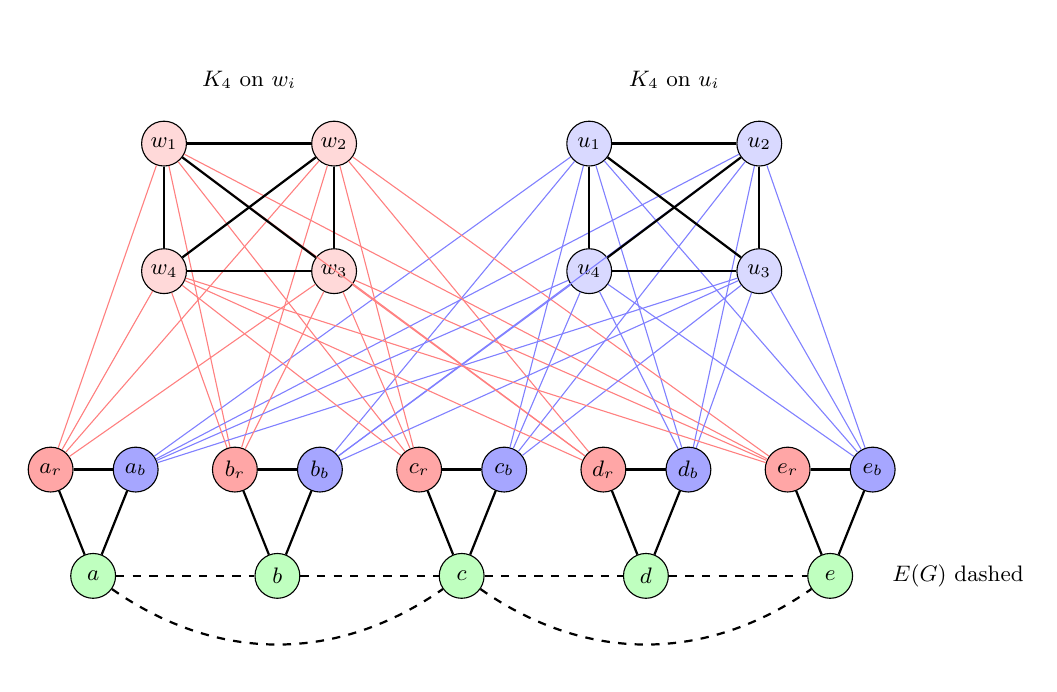
\begin{tikzpicture}[scale=0.9, transform shape,
          every node/.style={circle,draw,inner sep=1.5pt,minimum
          size=18pt,font=\small},
          wnode/.style={fill=red!15},
          unode/.style={fill=blue!15},
          rnode/.style={fill=red!35},
          bnode/.style={fill=blue!35},
          vnode/.style={fill=green!25},
          kedge/.style={thick},
          redge/.style={red!50,thin},
          bedge/.style={blue!50,thin},
          pedge/.style={thick},
          gedge/.style={thick,dashed}
        ]

        % --- K4 on w_1,...,w_4 (left) ---
        \node[wnode] (w1) at (-4.2, 4.6) {$w_1$};
        \node[wnode] (w2) at (-1.8, 4.6) {$w_2$};
        \node[wnode] (w3) at (-1.8, 2.8) {$w_3$};
        \node[wnode] (w4) at (-4.2, 2.8) {$w_4$};

        % --- K4 on u_1,...,u_4 (right) ---
        \node[unode] (u1) at ( 1.8, 4.6) {$u_1$};
        \node[unode] (u2) at ( 4.2, 4.6) {$u_2$};
        \node[unode] (u3) at ( 4.2, 2.8) {$u_3$};
        \node[unode] (u4) at ( 1.8, 2.8) {$u_4$};

        % --- for each v in V(G): v_r, v_b, and v ---
        \foreach \v/\x in {a/-5.2, b/-2.6, c/0, d/2.6, e/5.2} {
          \node[rnode] (\v r) at (\x-0.6, 0)   {$\v_r$};
          \node[bnode] (\v b) at (\x+0.6, 0)   {$\v_b$};
          \node[vnode] (\v)   at (\x,    -1.5) {$\v$};
        }

        % --- edges w_i -- v_r and u_i -- v_b (underneath) ---
        \foreach \i in {1,2,3,4}
        \foreach \v in {a,b,c,d,e} {
          \draw[redge] (w\i) -- (\v r);
          \draw[bedge] (u\i) -- (\v b);
        }

        % --- K4 edges ---
        \foreach \i/\j in {1/2,1/3,1/4,2/3,2/4,3/4} {
          \draw[kedge] (w\i) -- (w\j);
          \draw[kedge] (u\i) -- (u\j);
        }

        % --- triangles v, v_r, v_b ---
        \foreach \v in {a,b,c,d,e} {
          \draw[pedge] (\v r) -- (\v b);
          \draw[pedge] (\v)   -- (\v r);
          \draw[pedge] (\v)   -- (\v b);
        }

        % --- edges of G: ab, bc, cd, de, ac, ce ---
        \draw[gedge] (a) -- (b);
        \draw[gedge] (b) -- (c);
        \draw[gedge] (c) -- (d);
        \draw[gedge] (d) -- (e);
        \draw[gedge] (a) to[bend right=35] (c);
        \draw[gedge] (c) to[bend right=35] (e);

        % labels
        \node[draw=none,fill=none] at (-3.0, 5.5) {$K_4$ on $w_i$};
        \node[draw=none,fill=none] at ( 3.0, 5.5) {$K_4$ on $u_i$};
        \node[draw=none,fill=none,anchor=west] at (6.0,-1.5) {$E(G)$ dashed};

      \end{tikzpicture}
    \end{center}
    Assume that $G$ has a proper $3$-colouring $c_G\colon V(G)\to\{0,1,2\}$.
    Define $c\colon V(G^\star)\to\{0,1,2,3,4\}$ by
    \[
      c(x) =
      \begin{cases}
        c_G(v) & \text{if } x = v \in V(G),\\[2pt]
        3      & \text{if } x = v_b \text{ for some } v \in V(G),\\[2pt]
        4      & \text{if } x = v_r \text{ for some } v \in V(G),\\[2pt]
        i-1    & \text{if } x = w_i,\ i\in\{1,2,3,4\},\\[2pt]
        i-1    & \text{if } x = u_i,\ i\in\{1,2,3\},\\[2pt]
        4      & \text{if } x = u_4.
      \end{cases},
    \]
    which yields a proper $5$-coloring on $G^\star.$

    Conversely, assume we have some proper $5$-coloring on $G^\star.$
    Since $v_r$ has edges to $w_1, \ldots, w_4$ and we have $5$ valid
    colors, $c(t_r)= c(v_r)$ for any $t, v \in V(G).$ We can make a
    similar argument for $v_b,$ and since we have edges $(v_r,v_b),$
    $c(v_r) \neq c(v_b).$ Hence, this eliminates the two colors
    $c(v_r)$ and $c(v_b)$ from the possible colors on the subgraph
    induced $V(G),$ meaning this subgraph has a valid $3$-coloring.
    Since $G$ and the subgraph induced by $V(G)$ on $G^\star$ are
    isomorphic, this means $G$ has a proper $3$-coloring.

    Thus, $G$ has a proper $3$-coloring iff $G^\star$ has a proper $5$-coloring.

    This reduction creates $2|V| + 8 = \Theta(|V|)$ new vertices, and
    $$\mathcal O(V)$$ new edges, meaning we can construct such a
    reduction in polynomial time. Hence, given a polynomial time
    oracle for $5$-coloring, we can solve $3$-coloring in polynomial
    time, meaning $5$-coloring is NP-hard.

    Additionally, $5$-coloring is in NP since we can verify whether
    an instance is a valid coloring in $\mathcal O(|E|)$ time by
    checking all edges and verifying that any two adjacent vertices
    have different colors.

    Thus, $5$-coloring is NP-complete.

  \item
    \begin{enumerate}
      \item Assume that "length" refers to the number of vertices
        along some path. If $G$ has a Hamiltonian path, then this
        path has length $n = \log n',$  meaning graph $G'$ has a path
        of length $\log n'.$

        Conversely, if $G'$ has a path of length $\log n' = n,$ given
        $n > 1,$ this path cannot contain any of the isolated
        vertices, meaning there is a path of length $n = |V(G)|$ over
        $V(G),$ and hence by definition this is a Hamiltonian path on
        $G.$ Otherwise, if $n = 1$ then trivially, both $G'$ has a
        $\log n' = 1$ path and $G$ contains a Hamiltonian path.

        Hence, $G$ has a Hamiltonian path iff $G'$ has a $\log n$-path.

      \item Reduction is exp-time, meaning we cannot conclude that
        $\log n$-path is NP hard.

      \item Inserting $n^{100} - n$ isolated vertices is a
        $n^{100}$-time (poly time) reduction, and doesn't have the
        same problem as (b) since the reduction is polynomial time,
        which allows us to conclude $n^{0.01}$-path is NP-hard.
    \end{enumerate}
\end{enumerate}
\end{document}
